\documentclass[tikz,border=6pt]{standalone}
\usepackage[T1]{fontenc}
\usepackage{tikz}
\usetikzlibrary{arrows.meta,positioning,fit,calc}

\definecolor{stageblue}{RGB}{45,90,160}
\definecolor{stagegreen}{RGB}{40,125,85}
\definecolor{stageorange}{RGB}{185,115,35}
\definecolor{stagepurple}{RGB}{115,75,150}
\definecolor{lightblue}{RGB}{232,240,252}
\definecolor{lightgreen}{RGB}{232,247,239}
\definecolor{lightorange}{RGB}{252,242,230}
\definecolor{lightpurple}{RGB}{243,237,250}
\definecolor{linegray}{RGB}{70,75,85}

\tikzset{
  stage/.style={rounded corners=2pt, draw=#1, very thick, fill=#1!8, align=center, minimum height=1.0cm, font=\sffamily\small},
  subbox/.style={rounded corners=2pt, draw=linegray!55, fill=white, align=center, minimum height=0.70cm, font=\sffamily\scriptsize},
  arrow/.style={-{Latex[length=2.3mm,width=1.6mm]}, thick, draw=linegray},
  softarrow/.style={-{Latex[length=2.0mm,width=1.4mm]}, semithick, draw=linegray!70},
  labeltext/.style={font=\sffamily\scriptsize, align=center, text=linegray}
}

\begin{document}
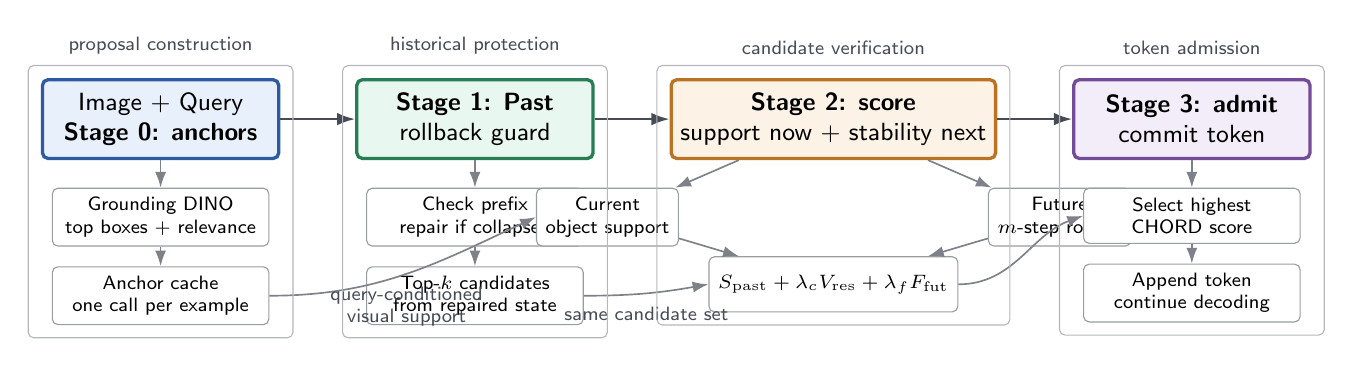
\begin{tikzpicture}[node distance=0.55cm and 0.75cm]

\node[stage=stageblue, fill=lightblue, minimum width=3.0cm] (input) {Image + Query\\\textbf{Stage 0: anchors}};
\node[subbox, below=0.35cm of input, minimum width=2.75cm] (dino) {Grounding DINO\\top boxes + relevance};
\node[subbox, below=0.25cm of dino, minimum width=2.75cm] (cache) {Anchor cache\\one call per example};

\node[stage=stagegreen, fill=lightgreen, right=0.95cm of input, minimum width=3.0cm] (past) {\textbf{Stage 1: Past}\\rollback guard};
\node[subbox, below=0.35cm of past, minimum width=2.75cm] (prefix) {Check prefix\\repair if collapsed};
\node[subbox, below=0.25cm of prefix, minimum width=2.75cm] (cand) {Top-$k$ candidates\\from repaired state};

\node[stage=stageorange, fill=lightorange, right=0.95cm of past, minimum width=3.2cm] (score) {\textbf{Stage 2: score}\\support now + stability next};
\node[subbox, below left=0.35cm and -0.12cm of score, minimum width=1.55cm] (current) {Current\\object support};
\node[subbox, below right=0.35cm and -0.12cm of score, minimum width=1.55cm] (future) {Future\\$m$-step rollout};
\node[subbox, below=1.22cm of score, minimum width=3.0cm] (aggregate) {$S_{\rm past}+\lambda_c V_{\rm res}+\lambda_f F_{\rm fut}$};

\node[stage=stagepurple, fill=lightpurple, right=0.95cm of score, minimum width=3.0cm] (admit) {\textbf{Stage 3: admit}\\commit token};
\node[subbox, below=0.35cm of admit, minimum width=2.75cm] (select) {Select highest\\CHORD score};
\node[subbox, below=0.25cm of select, minimum width=2.75cm] (next) {Append token\\continue decoding};

\draw[arrow] (input) -- (past);
\draw[arrow] (past) -- (score);
\draw[arrow] (score) -- (admit);

\draw[softarrow] (input) -- (dino);
\draw[softarrow] (dino) -- (cache);
\draw[softarrow] (past) -- (prefix);
\draw[softarrow] (prefix) -- (cand);
\draw[softarrow] (score) -- (current);
\draw[softarrow] (score) -- (future);
\draw[softarrow] (current) -- (aggregate);
\draw[softarrow] (future) -- (aggregate);
\draw[softarrow] (admit) -- (select);
\draw[softarrow] (select) -- (next);

\draw[softarrow] (cache.east) to[out=0,in=205] node[labeltext, below, yshift=-0.04cm] {query-conditioned\\visual support} (current.west);
\draw[softarrow] (cand.east) to[out=0,in=190] node[labeltext, below, yshift=-0.05cm] {same candidate set} (aggregate.west);
\draw[softarrow] (aggregate.east) to[out=0,in=200] (select.west);

\node[labeltext, above=0.18cm of input] {proposal construction};
\node[labeltext, above=0.18cm of past] {historical protection};
\node[labeltext, above=0.18cm of score] {candidate verification};
\node[labeltext, above=0.18cm of admit] {token admission};

\node[draw=linegray!40, rounded corners=2pt, fit=(input)(cache), inner sep=0.16cm] {};
\node[draw=linegray!40, rounded corners=2pt, fit=(past)(cand), inner sep=0.16cm] {};
\node[draw=linegray!40, rounded corners=2pt, fit=(score)(aggregate), inner sep=0.16cm] {};
\node[draw=linegray!40, rounded corners=2pt, fit=(admit)(next), inner sep=0.16cm] {};

\end{tikzpicture}
\end{document}
